
\section{Real time scheduling}
\label{sec:sched-rt}

There is a way to configure tasks so that Linux enforces global priorities:
processes that run in real time have strict priority over other processes, and
are under a different scheduler that enforces strict and global priorities among
the real time threads.

Linux implements real time scheduling alongside the usual weighted fair share by
supporting different \textit{scheduling classes}. There are three scheduling
classes that are accessible to users, listed in descending order of priority:
Deadline, Fifo, and Normal. Generally speaking most load is expected to fall
into the Normal scheduling class (hence the name). It is the default scheduling
class, and it is only within the Normal scheduling class that the cgroup
cpu.weight interface is relevant.

Each scheduling class exists completely separately: classes maintain their own
run queues and per-entity state; implement their own scheduling algorithms to
choose from the entities on their runqueue; and balance the load across
runqueues on different cores.

Linux isolates strictly between different scheduling classes: it only schedules
a lower scheduling class if the higher scheduling classes found nothing to run,
and each scheduling class tries to steal work from other cores before returning
that it has nothing to run. It is thereby true that if something in the Normal
scheduling class is running, it means there are no Fifo tasks waiting to run
anywhere on the machine.

\begin{figure*}[t]
    \centering
    \begin{subfigure}[t]{0.48\textwidth}
        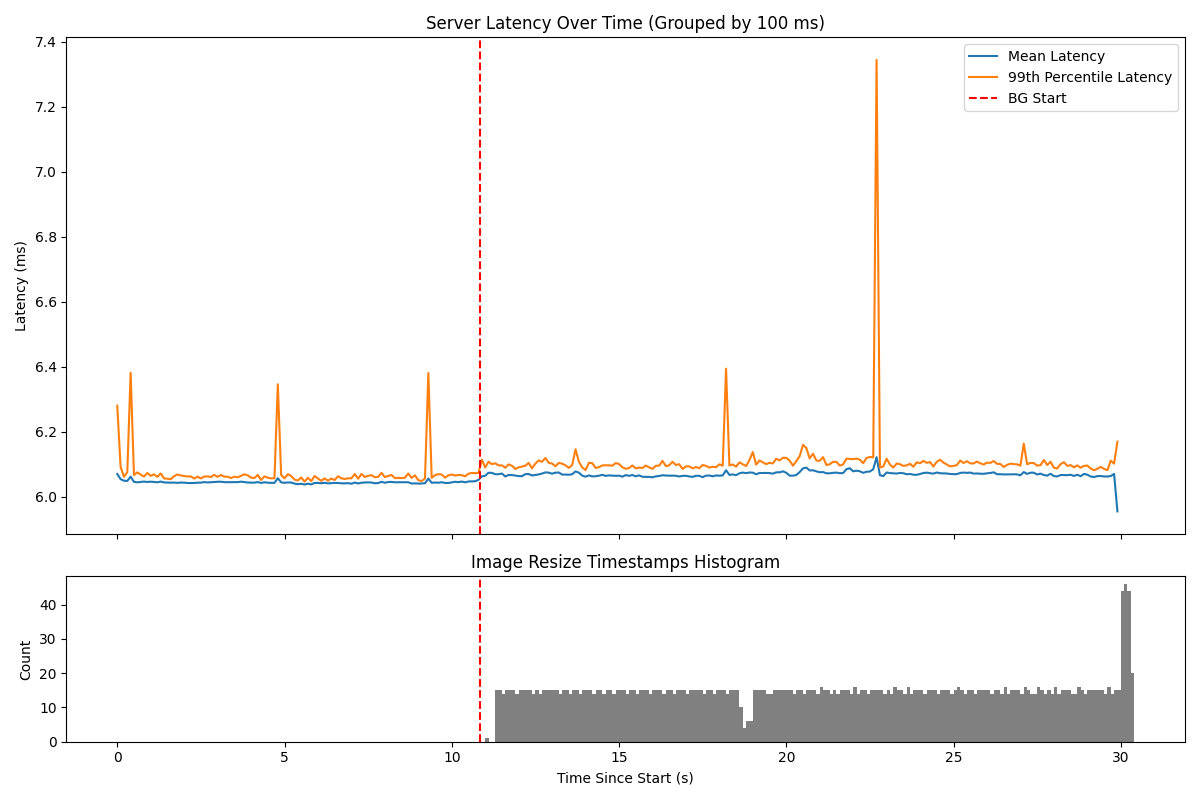
\includegraphics[width=\textwidth]{graphs/unedited-rt-low-two.png}
        \caption{Low load}\label{fig:unedited-rt-low-two}
    \end{subfigure}
    \hspace{\fill}
    \begin{subfigure}[t]{0.48\textwidth}
        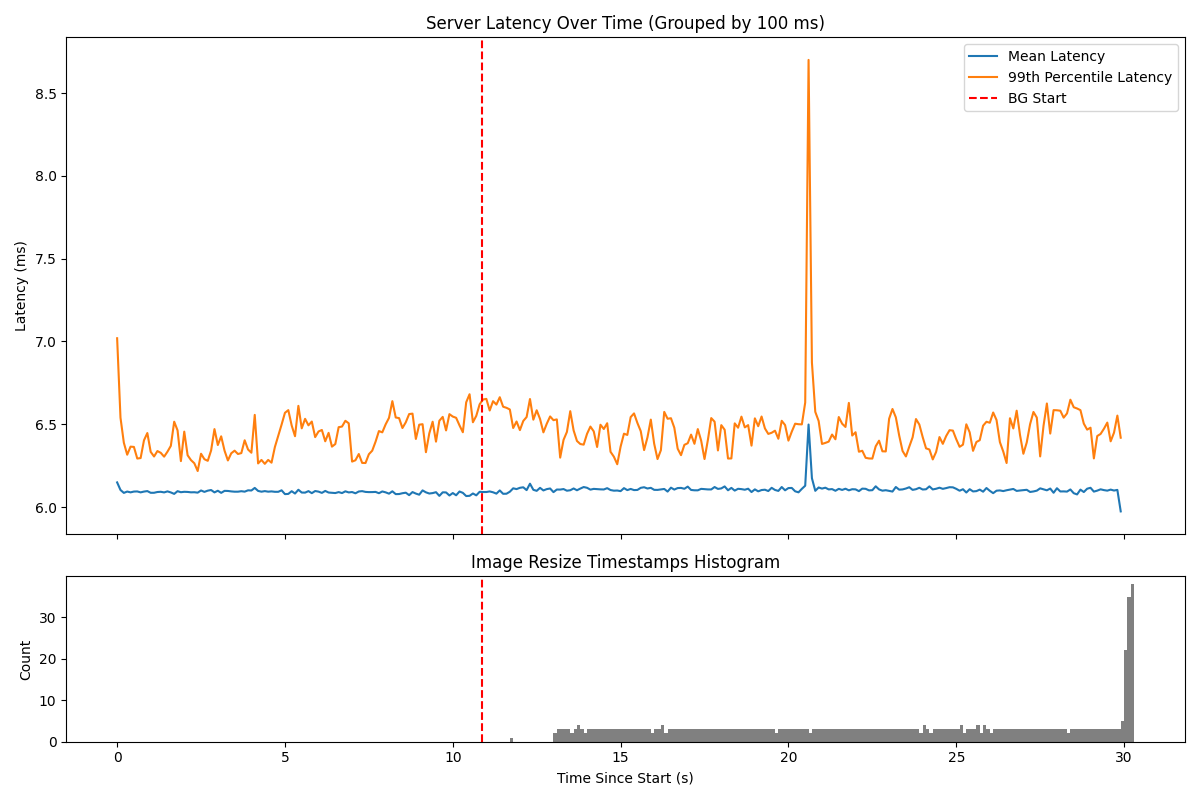
\includegraphics[width=\textwidth]{graphs/unedited-rt-high-two.png}
        \caption{High load}\label{fig:unedited-rt-high-two}
    \end{subfigure}
    \caption{Results of the same experiment, with LC running as a real time process}\label{fig:unedited-rt}
\end{figure*}

This points to a possible solution: run LC in Fifo and BE in Normal. Doing so
effectively promotes the latency criticality of the LC task in the eyes of the
system, and makes use of Linux's strong isolation of real time workloads.
Figure~\ref{fig:unedited-rt} shows the resulting measured latencies in the same
low and high load setting as previously. We see much stabler latencies, as
expected; in the baseline as well as once the BE tasks are started. This looks
promising on two fronts: 1: we get better isolation by making use of Linux's
strict boundaries between scheduling classes, and 2: we see improved tail
latency for the LC task by using a fifo run-to-completion scheduling algorithm.

However, the first benefit of improved stability comes at a cost. Because the
global ordering is so strict, also within the Fifo scheduling class, Linux is
performing balancing and potentially migration almost every time an LC thread
wakes up or exits. This requires the scheduling core to potentially lock the
runqueues of all the other cores as it ensures the task it will run the next is
the one with the highest priority, and within that priority the once that first
became runnable. This increase in scheduling latency leads to the small increase
in the baseline latency that is visible in the graphs.

And second benefit, the observed improved tail latency, is a side-effect of the
experimental setup, where each request does the exact same thing and processing
times are uniform. This is not true for a production environment, where request
processing times are variable and unknown. If a fifo run-to-completion scheduler
is used in that setting, it leads to HoL blocking, and thus to much worse tail
latencies for short requests.

We conclude that the Fifo scheduling class is not a good solution: although it
is able to globally ensure isolation between LC and BE tasks, its scheduling
time overheads and algorithm make in poorly suited for a production setting.



